\documentclass[10pt,a4paper]{article}
\usepackage[UTF8,fontset = windows]{ctex}
\setCJKmainfont[BoldFont=黑体,ItalicFont=楷体]{华文中宋}
\usepackage{amssymb,amsmath,amsfonts,amsthm,mathrsfs,dsfont,graphicx}
\usepackage{ifthen,indentfirst,enumerate,color,titletoc}
\usepackage{tikz}
\usepackage{multicol}
\usepackage{makecell}
\usepackage{longtable}
\usetikzlibrary{arrows,calc,intersections,patterns,decorations.pathreplacing,3d,angles,quotes}
\usepackage[bf,small,indentafter,pagestyles]{titlesec}
\usepackage[top=1in, bottom=1in,left=0.8in,right=0.8in]{geometry}
\renewcommand{\baselinestretch}{1.65}
\newtheorem{defi}{定义~}
\newtheorem{eg}{例~}
\newtheorem{ex}{~}
\newtheorem{rem}{注~}
\newtheorem{thm}{定理~}
\newtheorem{coro}{推论~}
\newtheorem{axiom}{公理~}
\newtheorem{prop}{性质~}
\newcommand{\blank}[1]{\underline{\hbox to #1pt{}}}
\newcommand{\bracket}[1]{(\hbox to #1pt{})}
\newcommand{\onech}[4]{\par\begin{tabular}{p{.9\textwidth}}
A.~#1\\
B.~#2\\
C.~#3\\
D.~#4
\end{tabular}}
\newcommand{\twoch}[4]{\par\begin{tabular}{p{.46\textwidth}p{.46\textwidth}}
A.~#1& B.~#2\\
C.~#3& D.~#4
\end{tabular}}
\newcommand{\vartwoch}[4]{\par\begin{tabular}{p{.46\textwidth}p{.46\textwidth}}
(1)~#1& (2)~#2\\
(3)~#3& (4)~#4
\end{tabular}}
\newcommand{\fourch}[4]{\par\begin{tabular}{p{.23\textwidth}p{.23\textwidth}p{.23\textwidth}p{.23\textwidth}}
A.~#1 &B.~#2& C.~#3& D.~#4
\end{tabular}}
\newcommand{\varfourch}[4]{\par\begin{tabular}{p{.23\textwidth}p{.23\textwidth}p{.23\textwidth}p{.23\textwidth}}
(1)~#1 &(2)~#2& (3)~#3& (4)~#4
\end{tabular}}
\begin{document}

\begin{enumerate}[1.]
\item 如图, 用集合语言描述下列图形中的点、直线、平面之间的位置关系.
\begin{center}
(1) 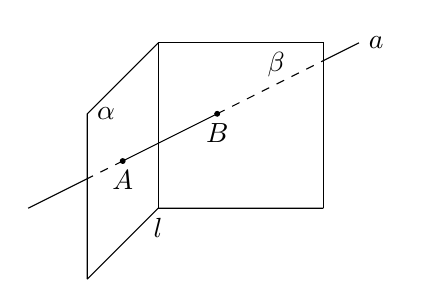
\begin{tikzpicture}[>=latex,scale = 1.5]
\draw (1,0.4) -- (1.6,1) -- (3,1);
\draw (1.6,1) -- (1.6,2.4);
\draw [name path = rightside] (3,1) -- (3,2.4) -- (1.6,2.4);
\draw [name path = leftside] (1,0.4) -- (1,1.8) -- (1.6,2.4);
\filldraw (1.3,1.4) circle (0.02) node [below] {$A$} coordinate (A) (2.1,1.8) circle (0.02) node [below] {$B$} coordinate (B);
\path [name path = leftline] ($(A)!-1!(B)$)  coordinate (S) -- (A);
\path [name path = rightline] ($(A)!2.5!(B)$) coordinate (T) -- (B);
\path [name intersections = {of = leftside and leftline, by = C}];
\path [name intersections = {of = rightside and rightline, by = D}];
\draw (D) -- (T) node [right] {$a$} (C) -- (S) (A) -- (B);
\draw [dashed] (A) -- (C) (B) -- (D);
\draw (1.6,1) node [below] {$l$};
\draw (1,1.8) node [right] {$\alpha$} (2.6,2.4) node [below] {$\beta$};
\end{tikzpicture}
(2) 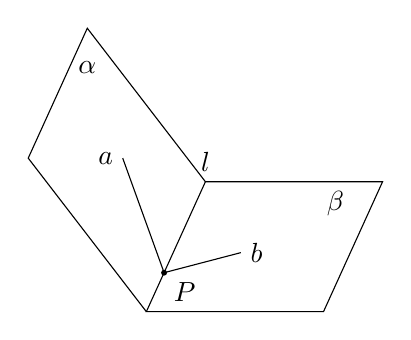
\begin{tikzpicture}[>=latex,scale = 1.5]
    \draw (1.2,0.4) coordinate (X) -- (2.7,0.4) -- (3.2,1.5) -- (1.7,1.5) coordinate (Y) -- cycle;
    \draw (X) -- (0.2,1.7) --++ (0.5,1.1)  -- (Y) node [above] {$l$};
    \draw (0.7,2.6) node [below] {$\alpha$} (2.8,1.5) node [below] {$\beta$};
    \filldraw ($(X)!0.3!(Y)$) circle (0.02) node [below right] {$P$} coordinate (T);
    \draw (T) -- (1,1.7) node [left] {$a$} (T) -- (2,0.9) node [right] {$b$};
    \end{tikzpicture}
\end{center}
\item 证明: 若四边形有三条边在一个平面上 , 则它的第四条边也在这个平面上. 
\item 已知$a$、$b$、$c$是空间的三条直线, $a\parallel b$, 且$c$与$a$、$b$
都相交. 求证: 直线$a$、$b$、$c$在同一平面上.
\item 如图, 在长方体$ABCD-A_1B_1C_1D_1$中, 画出$A_1B$与$A$、$B_1$、$C$所确定的平面的交点, 并说明理由.
\begin{center}
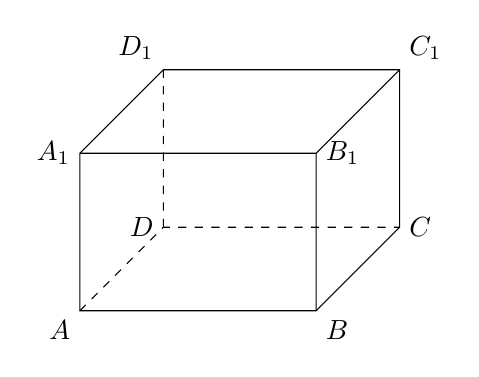
\begin{tikzpicture}[>=latex]
\draw (0,0) node [below left] {$A$} coordinate (A) --++ (3,0) node [below right] {$B$} coordinate (B) --++ (45:{3/2}) node [right] {$C$} coordinate (C)
--++ (0,2) node [above right] {$C_1$} coordinate (C1)
--++ (-3,0) node [above left] {$D_1$} coordinate (D1) --++ (225:{3/2}) node [left] {$A_1$} coordinate (A1) -- cycle;
\draw (A) ++ (3,2) node [right] {$B_1$} coordinate (B1) -- (B) (B1) --++ (45:{3/2}) (B1) --++ (-3,0);
\draw [dashed] (A) --++ (45:{3/2}) node [left] {$D$} coordinate (D) --++ (3,0) (D) --++ (0,2);
\end{tikzpicture}
\end{center}
\item 如何用绳子检查桌椅的四个脚是否立于同一平面上? 给出方案并说明理由. 
\item 画三个平面, 使其中的两个平面互相平行, 而第三个平面与这两个平面都相交.
\item 用硬纸板作为平面的模型, 摆出三个平面两两相交各种不同的情况.
\item 如图, 在长方体$ABCD-A_1B_1C_1D_1$中,
\begin{center}
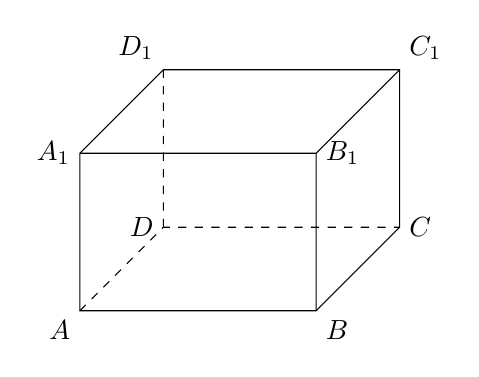
\begin{tikzpicture}[>=latex]
\draw (0,0) node [below left] {$A$} coordinate (A) --++ (3,0) node [below right] {$B$} coordinate (B) --++ (45:{3/2}) node [right] {$C$} coordinate (C)
--++ (0,2) node [above right] {$C_1$} coordinate (C1)
--++ (-3,0) node [above left] {$D_1$} coordinate (D1) --++ (225:{3/2}) node [left] {$A_1$} coordinate (A1) -- cycle;
\draw (A) ++ (3,2) node [right] {$B_1$} coordinate (B1) -- (B) (B1) --++ (45:{3/2}) (B1) --++ (-3,0);
\draw [dashed] (A) --++ (45:{3/2}) node [left] {$D$} coordinate (D) --++ (3,0) (D) --++ (0,2);
\end{tikzpicture}
\end{center}
(1) 设$AC$与$BD$的交点为$O$, $O$必为平面\blank{50}与平面\blank{50}的公共点(答案不唯一);\\
(2) 画出平面$A_1BCD_1$与平面$B_1BDD_1$的交线. 
\item 在水平放置的平面上有一个边长为$3\text{cm}$的正三角形, 请画出其直观图.
\item 画出如图水平放置的直角梯形$OABC$的直观图.
\begin{center}
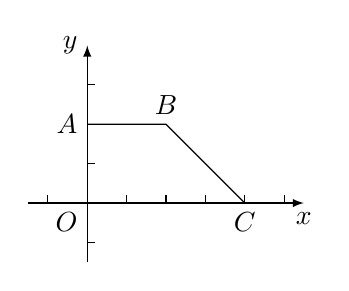
\begin{tikzpicture}[>=latex,scale = 0.5]
\draw [->] (-1.5,0) -- (5.5,0) node [below] {$x$};
\draw [->] (0,-1.5) -- (0,4) node [left] {$y$};
\draw (0,0) node [below left] {$O$};
\foreach \i in {-1,1,2,3,4,5} {\draw (\i,0.2) -- (\i,0);};
\foreach \i in {-1,1,2,3} {\draw (0.2,\i) -- (0,\i);};
\draw (4,0) node [below] {$C$} -- (2,2) node [above] {$B$} -- (0,2) node [left] {$A$};
\end{tikzpicture}
\end{center}
\item 如图, 在长方体$ABCD-A_1B_1C_1D_1$中, 直线$A_1C$与$BD_1$相交吗? 为什么?
\begin{center}
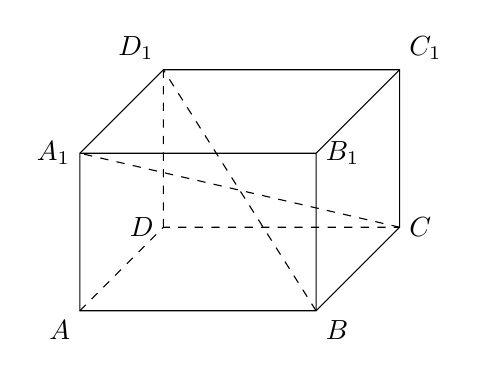
\begin{tikzpicture}[>=latex]
\draw (0,0) node [below left] {$A$} coordinate (A) --++ (3,0) node [below right] {$B$} coordinate (B) --++ (45:{3/2}) node [right] {$C$} coordinate (C)
--++ (0,2) node [above right] {$C_1$} coordinate (C1)
--++ (-3,0) node [above left] {$D_1$} coordinate (D1) --++ (225:{3/2}) node [left] {$A_1$} coordinate (A1) -- cycle;
\draw (A) ++ (3,2) node [right] {$B_1$} coordinate (B1) -- (B) (B1) --++ (45:{3/2}) (B1) --++ (-3,0);
\draw [dashed] (A) --++ (45:{3/2}) node [left] {$D$} coordinate (D) --++ (3,0) (D) --++ (0,2);
\draw [dashed] (B) -- (D1) (C) -- (A1);
\end{tikzpicture}
\end{center}
\item 在如图所示的长方体$ABCD-A_1B_1C_1D_1$中, 平面$A_1B_1C_1D_1$上
有一条直线$MN$, 而平面$ABCD$上有一点$P$. 试过点$P$作一条直线$l$, 使得$l\parallel MN$.
\begin{center}
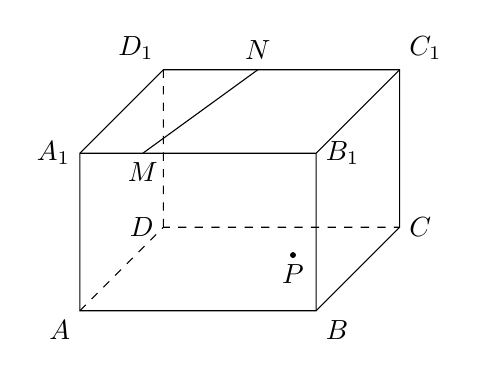
\begin{tikzpicture}[>=latex]
\draw (0,0) node [below left] {$A$} coordinate (A) --++ (3,0) node [below right] {$B$} coordinate (B) --++ (45:{3/2}) node [right] {$C$} coordinate (C)
--++ (0,2) node [above right] {$C_1$} coordinate (C1)
--++ (-3,0) node [above left] {$D_1$} coordinate (D1) --++ (225:{3/2}) node [left] {$A_1$} coordinate (A1) -- cycle;
\draw (A) ++ (3,2) node [right] {$B_1$} coordinate (B1) -- (B) (B1) --++ (45:{3/2}) (B1) --++ (-3,0);
\draw [dashed] (A) --++ (45:{3/2}) node [left] {$D$} coordinate (D) --++ (3,0) (D) --++ (0,2);
\draw (0.8,2) node [below] {$M$} -- ($(C1)!0.6!(D1)$) node [above] {$N$};
\filldraw (2,0) ++ (45:1) circle (0.03) node [below] {$P$};
\end{tikzpicture}
\end{center}
\item 如图, 在两个相交平面$\alpha$、$\beta$的交线上任意取两点$O$与$O_1$. 在平面$\alpha$上, 过$O$与$O_1$分别作射线$OA$与$O_1A_1$垂直于$OO_1$; 在平面$\beta$上, 过$O$与$O_1$分别作射线$OB$与$O_1B_1$垂直于$OO_1$. 求证: $\angle AOB=\angle A_1O_1B_1$.
\begin{center}
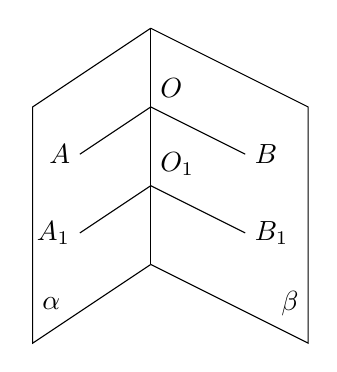
\begin{tikzpicture}[>=latex]
\draw (0,0) --++ (0,1) node [above right] {$O_1$} coordinate (O1) --++ (0,1) node [above right] {$O$} coordinate (O) --++ (0,1) coordinate (T);
\draw (T) --++ (-1.5,-1) --++ (0,-3) coordinate (BL) -- (0,0);
\draw (T) --++ (2,-1) --++ (0,-3) coordinate (BR) -- (0,0);
\draw (O1) --++ (-0.9,-0.6) node [left] {$A_1$};
\draw (O) --++ (-0.9,-0.6) node [left] {$A$};
\draw (O1) --++ (1.2,-0.6) node [right] {$B_1$};
\draw (O) --++ (1.2,-0.6) node [right] {$B$};
\draw (BL) ++ (0,0.5) node [right] {$\alpha$};
\draw (BR) ++ (0,0.5) node [left] {$\beta$};
\end{tikzpicture}
\end{center}
\item 在教室里找出几对异面直线的例子.
\item 如果一条直线和两条异面直线中的一条平行, 那么它和另一条直线的位置关
系是\blank{50}.
\item 下页左图是一个正方体的平面展开图, 请在下页右图的正方体中画出对应的线段, 并指出正方体中的线段$CN$、$AF$、$BM$、$ME$中, 哪些线段所在的直线与$DN$所在的直线是异面直线. 
\begin{center}
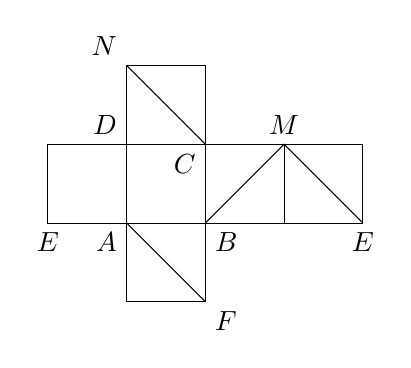
\begin{tikzpicture}[>=latex]
\draw (0,0) rectangle (4,1) (1,-1) rectangle (2,2) (3,0) -- (3,1);
\draw (0,0) node [below] {$E$} (1,0) node [below left] {$A$} (2,0) node [below right] {$B$} (4,0) node [below] {$E$};
\draw (1,1) node [above left] {$D$} (1,2) node [above left] {$N$} (3,1) node [above] {$M$} (2,-1) node [below right] {$F$} (2,1) node [below left] {$C$};
\draw (2,1) -- (1,2) (1,0) -- (2,-1) (2,0) -- (3,1) -- (4,0);
\end{tikzpicture}
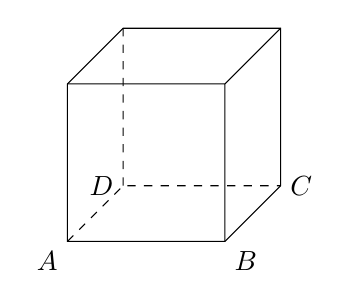
\begin{tikzpicture}[>=latex]
\draw (0,0) node [below left] {$A$} coordinate (A) --++ (2,0) node [below right] {$B$} coordinate (B) --++ (45:{2/2}) node [right] {$C$} coordinate (C)
--++ (0,2)  coordinate (C1)
--++ (-2,0)   coordinate (D1) --++ (225:{2/2}) coordinate (A1) -- cycle;
\draw (A) ++ (2,2)   coordinate (B1) -- (B) (B1) --++ (45:{2/2}) (B1) --++ (-2,0);
\draw [dashed] (A) --++ (45:{2/2}) node [left] {$D$} coordinate (D) --++ (2,0) (D) --++ (0,2);
\end{tikzpicture}
\end{center}
\item 在长方体$ABCD-A_1B_1C_1D_1$中, 与棱$AA_1$所在直线异面且垂直的棱有几条?
\item 在如图所示的正方体$ABCD-A_1B_1C_1D_1$中, 设$P$、$Q$分别是棱$BB_1$、$B_1C_1$的中点. 请画出异面直线$BD_1$与$PQ$所成的角.
\begin{center}
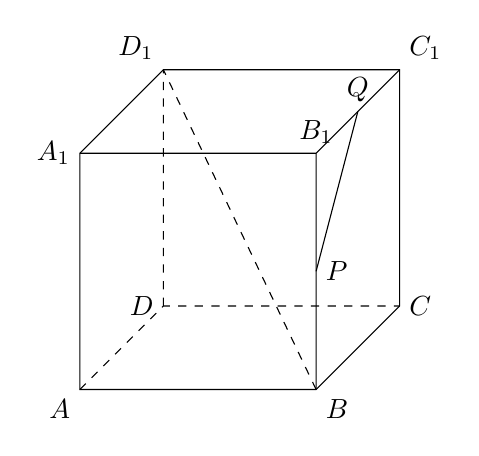
\begin{tikzpicture}[>=latex,scale = 1.5]
\draw (0,0) node [below left] {$A$} coordinate (A) --++ (2,0) node [below right] {$B$} coordinate (B) --++ (45:{2/2}) node [right] {$C$} coordinate (C)
--++ (0,2) node [above right] {$C_1$} coordinate (C1)
--++ (-2,0) node [above left] {$D_1$} coordinate (D1) --++ (225:{2/2}) node [left] {$A_1$} coordinate (A1) -- cycle;
\draw (A) ++ (2,2) node [above] {$B_1$} coordinate (B1) -- (B) (B1) --++ (45:{2/2}) (B1) --++ (-2,0);
\draw [dashed] (A) --++ (45:{2/2}) node [left] {$D$} coordinate (D) --++ (2,0) (D) --++ (0,2);
\draw [dashed] (B) -- (D1);
\draw ($(B)!0.5!(B1)$) node [right] {$P$} -- ($(B1)!0.5!(C1)$) node [above] {$Q$};
\end{tikzpicture}
\end{center}
\item 如图, 在长方体$ABCD-A_1B_1C_1D_1$的$6$个面中,
\begin{center}
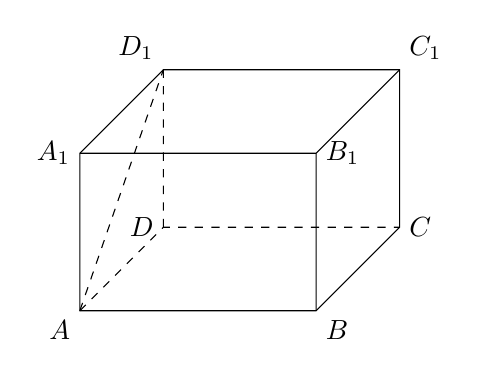
\begin{tikzpicture}[>=latex]
\draw (0,0) node [below left] {$A$} coordinate (A) --++ (3,0) node [below right] {$B$} coordinate (B) --++ (45:{3/2}) node [right] {$C$} coordinate (C)
--++ (0,2) node [above right] {$C_1$} coordinate (C1)
--++ (-3,0) node [above left] {$D_1$} coordinate (D1) --++ (225:{3/2}) node [left] {$A_1$} coordinate (A1) -- cycle;
\draw (A) ++ (3,2) node [right] {$B_1$} coordinate (B1) -- (B) (B1) --++ (45:{3/2}) (B1) --++ (-3,0);
\draw [dashed] (A) --++ (45:{3/2}) node [left] {$D$} coordinate (D) --++ (3,0) (D) --++ (0,2);
\draw [dashed] (A) -- (D1);
\end{tikzpicture}
\end{center}
(1) 与$AB$平行的平面是\blank{50};\\
(2) 与$AD_1$平行的平面是\blank{50}.
\item 判断下列命题的真假, 并说明理由:\\
(1) 若直线$a$上有无数个点不在平面$\alpha$上, 则$a\parallel \alpha$;\\
(2) 若直线$a$与平面$\alpha$上的一条直线平行, 则$a$与平面$\alpha$上的任意一条直线都平行;\\
(3) 若两条平行直线中的一条平行于一个平面, 则另一条直线也平行于这个平面;\\
(4) 设直线$a$在平面$\alpha$上, 直线$b$不在平面$\alpha$上, 并且$a\parallel b$, 则$b\parallel \alpha$.
\item 若直线$l$不平行于平面$\alpha$, 且$l$不在平面$\alpha$上, 判断下列结论是否成立, 并说明理由:\\
(1) 平面$\alpha$上的所有直线都与$l$异面;\\
(2) 平面$\alpha$上不存在与$l$平行的直线;\\
(3) 平面$\alpha$上存在唯一的一条直线与$l$平行;\\
(4) 平面$\alpha$上的直线都与$l$相交. 
\item 判断下列命题的真假, 并说明理由:\\
(1) 若两直线$a$、$b$互相平行, 则$a$平行于经过$b$的任何平面;\\
(2) 若直线$a$与平面$\alpha$平行, 则$a$平行于$\alpha$内的任何直线;\\
(3) 若两直线$a$、$b$都与平面$\alpha$平行, 则$a\parallel b$;\\
(4) 若直线$a$平行于平面$\alpha$, 直线$b$在平面$\alpha$上, 则$a\parallel b$或者$a$与$b$为异面直线.
\item 证明: 若不在给定平面上的两条平行直线中的一条平行于给定平面, 则另一条直线也平行于给定平面.
\item 设直线$a\parallel$平面$\alpha$, 求证: 过$a$任意作与$\alpha$相交的平面, 所有这些平面与$\alpha$的交线都是平行的. 
\item 加工六角螺母, 只要螺母的六个侧面都是矩形, 那么六条侧棱一定都垂直于螺母的上下两面. 请说明理由.
\item 设$AB$和$CD$都是平面$\alpha$的垂线, 其垂足分别为$B$、$D$. 已知$AB=2\text{cm}$, $CD=5\text{cm}$, $BD=4\text{cm}$. 求线段$AC$的长.
\item 如图, 已知$PA$垂直于平面$\alpha$, $PB$垂直于平面$\beta$, $A$、$B$为相应的垂足, 且$l$为平面$\alpha$与平面$\beta$的交线. 求证: $l\perp$平面$PAB$.
\begin{center}
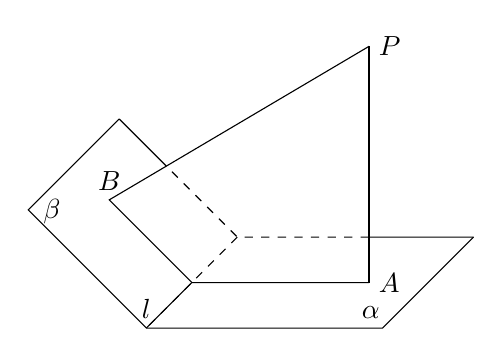
\begin{tikzpicture}[>=latex, scale = 1.5]
\draw (0,0,0) coordinate (O) (2,0,0) coordinate (R) (-1,1,0) coordinate (L);
\draw (O) ++ (0,0,2) coordinate (O1) (R) ++ (0,0,2) coordinate (R1) (L) ++ (0,0,2) coordinate (L1);
\draw (L) -- (L1) -- (O1) -- (R1) -- (R);
\path [name path = OR] (O) -- (R);
\path [name path = OL] (O) -- (L);
\draw [name path = AP] (1.5,0,1) node [right] {$A$} coordinate (A) --++ (0,2,0) node [right] {$P$} coordinate (P);
\draw [name path = BP] (A) --++ (-1.5,0,0) coordinate (O2) --++ (-0.7,0.7,0) node[above] {$B$} coordinate (B) -- (P);
\draw [name intersections = {of  = AP and OR, by = T}];
\draw [name intersections = {of  = BP and OL, by = S}];
\draw (O2) -- (O1) (T) -- (R) (S) -- (L);
\draw [dashed] (O) -- (O1) (T) -- (O) -- (S);
\draw (1.9,0,2) node [above] {$\alpha$} (L1) ++ (0.2,-0.2,0) node [above] {$\beta$} (O1) node [above] {$l$};
\end{tikzpicture}
\end{center}
\item 已知斜线段的长度是斜线段在平面内的投影的长的两倍, 求这条斜线和这个平面所成的角的大小.
\item 在正方体$ABCD-A_1B_1C_1D_1$中, $E$是边$A_1D_1$的中点.\\
(1) 求$A_1C$和底面$ABCD$所成角的大小;\\
(2) 求$EB$和底面$A_1B_1C_1D_1$所成角的大小.
\item 如图, 平面$\alpha$上的斜线$l$与平面$\alpha$所成的角为$\theta$, $l'$是$l$在平面$\alpha$上的投影, $O$是$l$与平面$\alpha$的交点, 点$B$是$l$上一点$A$在$\alpha$上的投影, $OC$是$\alpha$上的任意一条直线. 如果$\theta =45^\circ$, $\angle BOC=45^\circ$, 求$\angle AOC$, 并验证$\angle AOC>\theta$.
\begin{center}
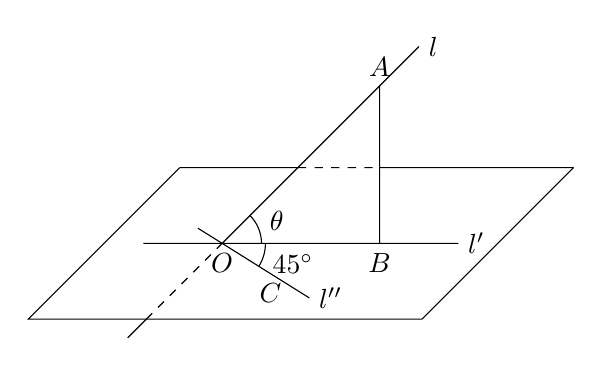
\begin{tikzpicture}[>=latex]
\draw (-1,0,0) -- (3,0,0) node [right] {$l'$} (2,2,0) node [above] {$A$} coordinate (A) -- (2,0,0) coordinate (B) node [below] {$B$} (2.5,2.5,0) node [right] {$l$} -- (0,0,0) coordinate (O) node [below] {$O$};
\draw (1,0,1) node [below] {$C$} coordinate (C);
\draw ($(O)!-0.5!(C)$) -- ($(O)!1.8!(C)$) node [right] {$l''$};
\draw [name path = edge] (-1.5,0,-2.5) coordinate (L) -- (-1.5,0,2.5) --++ (5,0,0) --++ (0,0,-5) coordinate (R);
\path [name path = LR] (L) -- (R);
\path [name path = OA] (O) -- (A);
\path [name path = AB] (A) -- (B);
\path [name intersections = {of = OA and LR, by = A1}];
\path [name intersections = {of = AB and LR, by = B1}];
\draw (L) -- (A1) (B1) -- (R);
\draw [dashed] (A1) -- (B1);
\path [name path = down] ($(O)!-0.6!(A)$) -- (O);
\path [name intersections = {of = down and edge, by = T}];
\draw (T) -- ($(O)!-0.6!(A)$);
\draw [dashed] (T) -- (O);
\draw (O) pic ["$\theta$",draw,angle eccentricity = 1.5] {angle = B--O--A};
\draw (O) pic ["$45^\circ$",scale = 1.1,draw,angle eccentricity = 1.7]{angle = C--O--B};
\end{tikzpicture}
\end{center}
\item 过$\triangle ABC$所在平面$\alpha$外的一点$P$, 作$PO\perp \alpha$, 垂足为$O$, 连接$PA$、$PB$及$PC$.\\
(1) 若$PA=PB=PC$, 则点$O$是$\triangle ABC$的\blank{50}心;\\
(2) 若$PA=PB=PC$, $\angle ACB=90^\circ$, 则点$O$是边$AB$的\blank{50}点;\\
(3) 若$PA\perp PB$, $PB\perp PC$, $PC\perp PA$, 则点$O$是$\triangle ABC$的\blank{50}心.
\item 已知$O$是$\triangle ABC$的垂心, 过点$O$作平面$ABC$的垂线, $P$是
垂线上的一点. 求证: $PA\perp BC$.
\item 如图, 已知$ABCD$是矩形, $PA\perp$平面$ABCD$.
\begin{center}
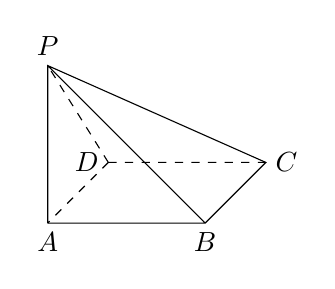
\begin{tikzpicture}[>=latex]
\draw (0,0,0) node [below] {$A$} coordinate (A) -- (2,0,0) node [below] {$B$} coordinate (B) -- (2,0,-2) node [right] {$C$} coordinate (C) -- (0,2,0) node [above] {$P$} coordinate (P) -- (A) (P) -- (B);
\draw [dashed] (0,0,-2)  node [left] {$D$} coordinate (D) -- (P) (D) --(A) (D) --(C);
\end{tikzpicture}
\end{center}
(1) 求证: $\angle PBC=90^\circ$;\\
(2) 若$PC\perp BD$, 求证: 四边形$ABCD$是正方形.
\item 判断下列命题的真假, 并说明理由:\\
(1) 若一个平面内的两条直线均平行于另一个平面, 则这两个平面平行;
(2) 若一个平面内两条不平行的直线都平行于另一个平面, 则这两个平面平行;
(3) 若两个平面平行, 则其中一个平面中的任何直线都平行于另一个平面;
(4) 平行于同一个平面的两个平面平行;
(5) 若一个平面内的任何一条直线都平行于另一个平面, 则这两个平面平行.
\item 如图, 已知正方体$ABCD-A_1B_1C_1D_1$的棱长为$a$, 求:
\begin{center}
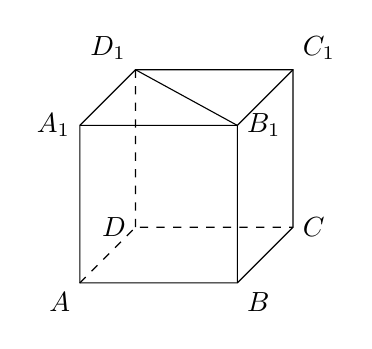
\begin{tikzpicture}[>=latex]
\draw (0,0) node [below left] {$A$} coordinate (A) --++ (2,0) node [below right] {$B$} coordinate (B) --++ (45:{2/2}) node [right] {$C$} coordinate (C)
--++ (0,2) node [above right] {$C_1$} coordinate (C1)
--++ (-2,0) node [above left] {$D_1$} coordinate (D1) --++ (225:{2/2}) node [left] {$A_1$} coordinate (A1) -- cycle;
\draw (A) ++ (2,2) node [right] {$B_1$} coordinate (B1) -- (B) (B1) --++ (45:{2/2}) (B1) --++ (-2,0);
\draw [dashed] (A) --++ (45:{2/2}) node [left] {$D$} coordinate (D) --++ (2,0) (D) --++ (0,2);
\draw (B1) -- (D1);
\end{tikzpicture}
\end{center}
(1) 点$A_1$到直线$BC$的距离;\\
(2) 点$A$到平面$B_1BCC_1$的距离;\\
(3) $B_1D_1$到平面$ABCD$的距离;\\
(4) 平面$B_1BCC_1$到平面$A_1ADD_1$的距离.
\item 证明: 夹在两个平行平面间的平行线段相等. 
\item 已知平面$\alpha\perp$平面$\beta$, 判断下列命题是否正确, 并说明理由:\\ 
(1) 平面$\alpha$上的任意一条直线都垂直于平面$\beta$上的任意一条直线;\\
(2) 平面$\alpha$上的任意一条直线都垂直于平面$\beta$上的无数条直线;\\
(3) 平面$\alpha$上的任意一条直线都垂直于平面$\beta$;\\
(4) 过平面$\alpha$上任意一点作平面$\alpha$与$\beta$交线的垂线$l$, 则$l\perp \beta$.
\item 如图, 已知$AB\perp$平面$BCD$, $BC\perp CD$, 有哪些平面互相
垂直? 为什么? 
\begin{center}
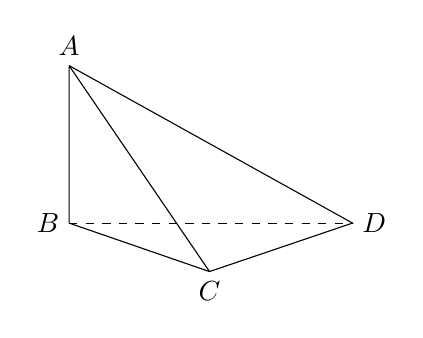
\begin{tikzpicture}[>=latex]
\draw (0,0,0) node [left] {$B$} coordinate (B) -- (2.4,0,1.6) node [below] {$C$} coordinate (C) -- (3.6,0,0) node [right] {$D$} coordinate (D) -- (0,2,0) node [above] {$A$} coordinate (A);
\draw (A) -- (B) (A) -- (C);
\draw [dashed] (B) -- (D); 
\end{tikzpicture}
\end{center}
\item 证明: 如果两个平面垂直, 那么过第一个平面上一点且垂直于第二个平面的直线, 必在第一个平面上. 
\item 如图, 设正方体$ABCDA_1B_1C_1D_1$的棱长为$1$, 求下列异面直线之间的距离:\\
\begin{center}
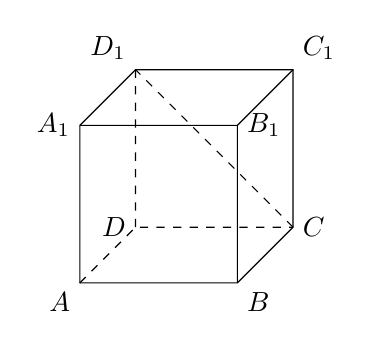
\begin{tikzpicture}[>=latex]
\draw (0,0) node [below left] {$A$} coordinate (A) --++ (2,0) node [below right] {$B$} coordinate (B) --++ (45:{2/2}) node [right] {$C$} coordinate (C)
--++ (0,2) node [above right] {$C_1$} coordinate (C1)
--++ (-2,0) node [above left] {$D_1$} coordinate (D1) --++ (225:{2/2}) node [left] {$A_1$} coordinate (A1) -- cycle;
\draw (A) ++ (2,2) node [right] {$B_1$} coordinate (B1) -- (B) (B1) --++ (45:{2/2}) (B1) --++ (-2,0);
\draw [dashed] (A) --++ (45:{2/2}) node [left] {$D$} coordinate (D) --++ (2,0) (D) --++ (0,2);
\draw [dashed] (C) -- (D1);
\end{tikzpicture}
\end{center}
(1) $AD$与$B_1B$;\\
(2) $AB$与$D_1C$.
\item 求两条异面直线之间的距离问题, 除了可转化为求直线与平面间的距离, 还可以转化为求两个平行平面之间的距离. 请给出两个平行平面的构造方法, 并说明为什么两条异面直线之间的距离就等于这样两个平行平面之间的距离.
\item 设两条电线所在的直线是异面直线, 它们的距离是$1\text{m}$, 所成的角是$60^\circ$. 已知这两条电线上各有一点, 距离公垂线的垂足都是$10\text{m}$. 求这两点之间的距离.
\item 证明: 棱柱的所有侧面都是平行四边形.
\item 证明: 平行于棱柱底面的平面截这个棱柱所得到的截面是一个与底面全等的多边形. 
\item 一个水平放置的封闭圆柱形容器中装了部分的水, 此时水面的形状是什么图形? 如果把圆柱沿侧面放倒在水平的面上, 那么水面的形状又会是什么图形? 请分别画出以上两种情形的示意图.
\item 在修建铁路时, 路基需要用碎石铺垫. 已知路基的形状及尺寸如图所示(单位: $\text{m}$), 每修建$1\text{km}$铁路需要碎石多少$\text{m}^3$?
\begin{center}
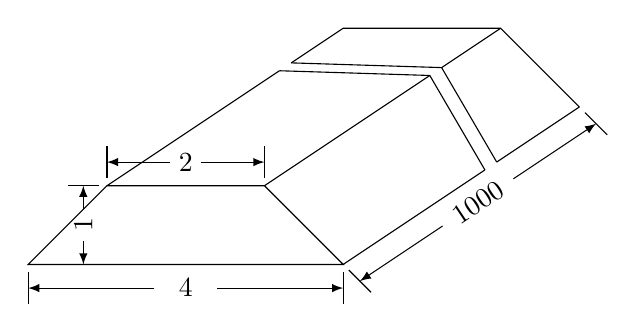
\begin{tikzpicture}[>=latex]
\draw (0,0) -- (4,0) coordinate (B)-- (3,1) coordinate (C)  -- (1,1) coordinate (D) -- cycle;
\path (D) ++ (3,2) coordinate (D1) (C) ++ (3,2) coordinate (C1) (B) ++ (3,2) coordinate (B1);
\path ($(B)!0.6!(B1)$) coordinate (B2) ($(C)!0.7!(C1)$) coordinate (C2) ($(D)!0.73!(D1)$) coordinate (D2);
\path ($(B)!0.65!(B1)$) coordinate (B3) ($(C)!0.75!(C1)$) coordinate (C3) ($(D)!0.78!(D1)$) coordinate (D3);
\draw (B) -- (B2) (B3) -- (B1) (C) -- (C2)  (C3) -- (C1) (D) -- (D2)  (D3) -- (D1);
\draw (B1) -- (C1) -- (D1) (B2) -- (C2) -- (D2) (B3) -- (C3) -- (D3);
\draw (0,-0.1) -- (0,-0.5) (4,-0.1) -- (4,-0.5);
\draw (2,-0.3) node {$4$};
\draw [->] (1.6,-0.3) -- (0,-0.3);
\draw [->] (2.4,-0.3) -- (4,-0.3);
\draw (4,0) ++ (-45:0.1) --++ (-45:0.4) (4,0) ++ (-45:0.3) coordinate (F);
\draw (7,2) ++ (-45:0.1) --++ (-45:0.4) (7,2) ++ (-45:0.3) coordinate (R);
\draw ($(F)!0.5!(R)$) node {\rotatebox{33.6901}{$1000$}};
\draw [->] ($(F)!0.35!(R)$) -- (F);
\draw [->] ($(F)!0.65!(R)$) -- (R);
\draw (0.5,1) -- (0.9,1);
\draw (0.7,0.5) node {\rotatebox{90}{$1$}};
\draw [->] (0.7,0.3) -- (0.7,0);
\draw [->] (0.7,0.7) -- (0.7,1);
\draw (1,1.1) -- (1,1.5) (3,1.1)-- (3,1.5);
\draw (2,1.3) node {$2$};
\draw [->] (1.8,1.3) -- (1,1.3);
\draw [->] (2.2,1.3) -- (3,1.3);
\end{tikzpicture}
\end{center}
\item 一个圆柱形油桶的底面半径为$50\text{cm}$, 高为$100\text{cm}$. 求这个油桶的体积.
\item 查一查六角螺帽的尺寸规格, 并说明如何计算它的体积. 
\item 如图(图中单位: $\text{cm}$)是一种机器零件, 零件下部是实心的直六棱
柱(底面是正六边形, 侧面是全等的矩形), 上部是实心的圆柱. 求此零件的体积与表面积. (结果分别精确到$0.1\text{cm}^3$与$0.1\text{cm}^2$)
\begin{center}
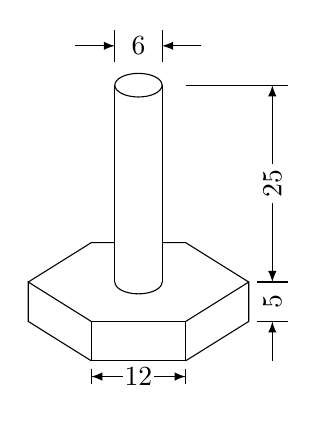
\begin{tikzpicture}[>=latex, scale = 0.1]
\draw (-6,0) -- (6,0) -- (6,5) -- (-6,5) -- cycle;
\draw (6,5) --++ (8,5) --++ (0,-5) -- (6,0);
\draw (-6,5) --++ (-8,5) coordinate (T) --++ (0,-5) -- (-6,0);
\draw (T) --++ (8,5) --++ (12,0) --++ (8,-5);
\draw (T) ++ (14,0) coordinate (O);
\filldraw [white] (O) ++ (3,0) rectangle++ (-6,25);
\draw (O) ++ (3,0) --++ (0,25);
\draw (O) ++ (-3,0) --++ (0,25);
\draw (O) ++ (3,0) arc (0:-180:3 and 1.5);
\draw (O) ++ (0,25) ellipse (3 and 1.5);
\draw (-6,-1) -- (-6,-3) (6,-1) -- (6,-3);
\draw [->] (-2,-2) -- (-6,-2);
\draw [->] (2,-2) -- (6,-2);
\draw (0,-2) node {$12$};
\draw (15,5) -- (19,5) (15,10) -- (19,10);
\draw (17,7.5) node {\rotatebox{90}{$5$}};
\draw [->] (17,0) -- (17,5);
\draw [->] (17,20) -- (17,10);
\draw [->] (17,25) -- (17,35);
\draw (6,35) -- (19,35);
\draw (17,22.5) node {\rotatebox{90}{$25$}};
\draw (-3,38) -- (-3,42) (3,38) -- (3,42);
\draw [->] (-8,40) -- (-3,40);
\draw [->] (8,40) -- (3,40);
\draw (0,40) node {$6$}; 
\end{tikzpicture}
\end{center}
\item 要给一批共$10000$根相同规格的空心钢管镀锌, 钢管的长度为
$1\text{m}$, 内外直径分别为$8\text{cm}$与$10\text{cm}$. 若电镀这批钢管每平方米要用锌$0.11\text{kg}$, 求需要用锌的总量. (结果精确到$0. 01\text{kg}$)
\item 证明: 表面积相等的长方体中, 正方体的体积最大.
\item 用平行于棱锥底面的平面截这个棱锥, 得到一个小棱锥. 已知这两个棱锥的高分别是$h_1$、$h_2$, 求这两个棱锥的底面面积之比.
\item (1) 过圆锥的任意两条母线作一个平面与圆锥相截, 得到的截面是什么图形?  在什么条件下, 所得到的截面面积最大? \\
(2) 如果圆锥的母线与底面所成的角为$60^\circ$, 那么经过圆锥两
条母线的平面与圆锥底面所成的二面角有可能小于$60^\circ$吗? 
\item 显然, 通过延长圆台的任意一条母线都可以使它们交于一点, 从而得到一个圆锥. 如图, 这样的几何体是否也可以通过延长棱的方法得到一个棱锥?
\begin{center}
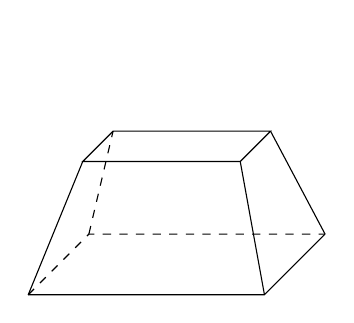
\begin{tikzpicture}[>=latex]
\draw (0,0,0) coordinate (A) -- (3,0,0) coordinate (B) --++ (0,0,-2) coordinate (C);
\draw [dashed] (0,0,0) -- (0,0,-2) coordinate (D) --++ (3,0,0);
\draw (1,3,-1) coordinate (S) (2,3,-1) coordinate (T);
\draw ($(A)!0.5!(S)$) coordinate (A1) ($(D)!0.5!(S)$) coordinate (D1) ($(C)!0.5!(T)$) coordinate (C1) ($(B)!0.5!(T)$) coordinate (B1);
\draw (A1) -- (B1) -- (C1) -- (D1) -- cycle;
\draw (A) -- (A1) (B) -- (B1) (C) -- (C1);
\draw [dashed] (D) -- (D1);
\end{tikzpicture}
\end{center}
\item 已知四棱锥$P-ABCD$的底面是边长为$6$的正方形, 侧棱$PA$垂直于底面, 且$PA=8$. 求该四棱锥的体积.
\item 已知直三棱柱$ABC-A'B'C'$的侧棱长为$9$, 底面相邻边的长分别是$7$和$5$, 夹角为$120^\circ$. 求三棱锥$B-A'B'C'$的体积.
\item 已知圆台上、下底面的半径分别为$r_1$、$r_2$, 高为$h$. 求证: $V_{\text{圆台}}=\dfrac 13\pi (r_1^2+r_1r_2+r_2^2)h$.
\item 已知圆锥侧面展开图中扇形的中心角为$\dfrac{2\pi}3$, 底面周长为$2\pi$. 求这个圆锥的侧面积和表面积.
\item 棱长都是$1$的三棱锥的表面积为\blank{50}.
\item 推导正棱台的侧面积公式.
\item 我国古代数学著作《九章算术》中研究过一种叫``鳖臑''的几何体(见《九章算术》卷第五``商功''之一六), 它指的是由四个直角三角形围成的四面体. 用你学过的立体几何知识说明这种四面体确实存在.
\item 有两个面平行, 其余各面都是平行四边形的多面体一定是柱体吗? 请给出你的理由或反例.
\item 一个置于地面上的救生圈是绕一条垂直于地平面的直线$l$旋转而成的旋转体.\\
(1) 如果用一个经过旋转轴$l$的平面去截这个生圈, 得到的截面是什么图形? 请画出示意图;\\
(2) 如果用一个平行于地面的平面去截这个救生圈, 得到的截面可能是什么图形? 请画出示意图.
\item $O$为球心,$O_1$为小圆的圆心, 用球的半径$r$和小圆的半径$r_1$表示$
OO_1$的距离$d$.
\item 已知半径为$R$的球面上三点$A$、$B$、$C$满足$AB=6$, $BC=8$, $CA=10$, 球心到平面$ABC$的距离为$12$. 求球的半径$R$.
\item 已知上海地处东经$120^\circ 52'$至$122^\circ 12'$, 北纬$30^\circ 40'$至$31^\circ 53'$之间, 地球半径为$6371.004\text{km}$. 求上海所辖区域:\\
(1) 经线对应的两平面所成的二面角的大小;\\
(2) 纬线所在两平面的距离.
\item 已知地球的半径约为$6371\text{km}$, 计算地球的表面积. (结果精确到
$10000\text{km}^2$)
\item 把一个半径为$R$的实心铁球熔化铸成两个小球, 两个小球的半径之比为$1:2$. 求其中较小球的半径.
\item 如图, 有一个水平放置的透明无盖的正方体容器, 容器高$8\text{cm}$, 将一个球放在容器口, 再向容器注水, 当球面恰好接触水面时, 测得水深为$
6\text{cm}$. 若不计容器的厚度, 求球的体积. 
\begin{center}
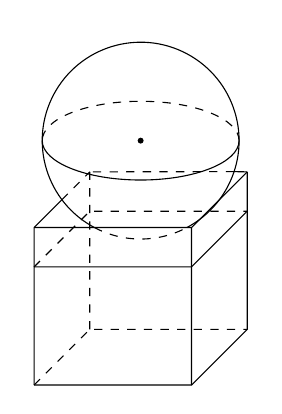
\begin{tikzpicture}[>=latex]
\draw (0,0)  coordinate (A) --++ (2,0)  coordinate (B) --++ (45:{2/2})  coordinate (C)
--++ (0,2)  coordinate (C1) ++ (-2,0)  coordinate (D1) ($(D1)!0.5!(0,2)$)--++ (225:{1/2})  coordinate (A1) -- (A);
\draw [dashed] ($(D1)!0.5!(0,2)$) -- (D1);
\draw (A) ++ (2,2)  coordinate (B1) -- (B) (B1) --++ (45:{2/2}) (B1) --++ (-2,0);
\draw [dashed] (A) --++ (45:{2/2})  coordinate (D) --++ (2,0) (D) --++ (0,2);
\draw (0,0) ++ (1,0) ++ (45:0.5) ++ (0,2) ++ (0,0.75) coordinate (O);
\draw (C1) -- (2.54,2.71);
\draw [dashed] (2.54,2.71) -- (D1);
\filldraw (O) circle (0.03);
\draw [dashed] (O) ++ (241.99:1.25) arc (241.99:298.01:1.25);
\draw (O) ++ (241.99:1.25) arc (241.99:{298.01-360}:1.25);
\draw (O) ++ (1.25,0) arc (0:-180:1.25 and 0.5);
\draw [dashed] (O) ++ (1.25,0) arc (0:180:1.25 and 0.5);
\draw (0,1.5) --++ (2,0) --++ (45:1);
\draw [dashed] (0,1.5) --++ (45:1) --++ (2,0);
\end{tikzpicture}
\end{center}
\item 判断下面哪些是随机现象, 哪些是确定性现象, 并列举几个生活中的确定性现象与随机现象的例子.\\
(1) 明天太阳升起;\\
(2) 明天上海局部地区下雨;\\
(3) 明年小明又大一岁;\\
(4) 小明今天放学回家到路口时恰好碰到绿灯.
\item 仿照正文中的例子分析下面两句话里含有怎样的随机性.\\
(1) 今年冬天一定会下雪;\\
(2) 今年我要参加高考, 应该能考上大学.
\item 按某个观察角度, 写出下面随机现象的一个样本空间:\\
(1) 抛掷$3$枚硬币;\\
(2) 将$3$个不同颜色的球放入$3$个不同的容器中, 但每个容器最多放$1$个球.
\item 掷一颗骰子, 写出样本空间及与下列事件相对应的基本事件子集:\\
(1) $1$没有出现;\\
(2) 出现奇数;\\
(3) 点数超过$2$.
\item 从两男两女四人中随机选出两人,\\
(1) 写出样本空间;\\
(2) 写出两人恰好是一男一女这个事件所对应的子集.
\item 同时掷$2$颗骰子, 求:\\
(1) 所得点数和为$6$的概率;\\
(2) 所得点数和不大于$6$的概率.
\item 抛掷$3$枚硬币, 求下列事件的概率:\\
(1) 恰有$2$枚正面朝上;\\
(2) 最多$1$枚正面朝上.
\item 掷两颗骰子, 点数之和出现哪个数的可能性最大?
\item (配对问题)三个人抽签, 三个签上事先分别写上了各自的名字. 求下面事件的概率:\\
$A_0$: 没有人抽到写有自己名字的签;\\
$A_1$: 恰有一个人抽到写有自己名字的签;\\
$A_2$: 恰有两个人抽到写有自己名字的签;\\
$A_3$: 三个人都抽到写有自己名字的签.
\item 写出例$6$中事件$A$、$B$各自包含的基本事件, 表示出$A\cup B$与$A\cap B$来验证例$6$中的结果.
\item 把$1$、$2$、$3$、$4$、$5$、$6$、$7$、$8$、$9$、$10$分别写在$10$张一样的卡片上, 并随机抽取$1$张. 设$A$: 出现偶数, $B$: 出现$3$的倍数. 写出下面两个事件的对应子集:\\
(1) $A$、$B$至少有一个发生;\\
(2) $A$、$B$同时发生. 
\item 已知$A$、$B$、$C$是三个两两互斥的事件, 求证: $P(A\cup B\cup C)=P(A)+P(B)+P(C)$.
\item 已知$A$、$B$是两个事件, 求证: $P(A\cap \overline B)=P(A)-P(A\cap B)$.
\item 一次期中考试, 小明数学超过$90$分的概率是$0.5$, 物理超过$90$分的概率是$0.7$, 两门课都超过$90$分的概率是$0.3$. 求他的数学和物理至少有一门超过$90$分的概率.
\item 早期破译密码, 注意文字的出现频率是一个重要手段. 找一篇(大约一页A4纸)英文文章, 计算一下$26$个英文字母出现的频率, 观察哪个字母出现的频率最高.
\item 有一批种子, 其中的种子可能$1$天发芽, 也可能$2$天发芽, $\cdots\cdots$, 下表是对不同发芽天数的种子数的记录.
\begin{center}
\begin{tabular}{|c|c|c|c|c|c|c|c|c|}
    \hline
    发芽次数/天 & $1$ & $2$ & $3$ & $4$ & $5$ & $6$ & $7$ & $\ge 8$\\ \hline
    种子数/粒 & $18$ & $36$ & $20$ & $11$ & $9$ & $3$ & $1$ & $0$ \\ \hline
\end{tabular}
\end{center}
(1) 求发芽天数为$2$天或$3$天的频率(经验概率);\\
(2) 求发芽天数超过$4$天的频率. (结果精确到$0.01$)
\item 管理人员为了了解某水库里大概有多少条鱼, 拖网打捞出$1000$条鱼, 在鱼身处打上一个不会掉落的印记, 再放回水库. 一个月后再次捕捞$1000$条鱼, 发现其中有$15$条有印记的鱼. 问: 这个水库里大概有多少条鱼?
\item 掷两颗骰子, 试用独立性求:\\
(1) 它们的点数都是偶数的概率;\\
(2) 它们的点数是一奇一偶的概率.
\item 已知事件$A$与事件$B$相互独立, 如果$P(A)=0.3$, $P(B)=0.6$, 那么$P(A\cap B)=$\blank{50}, $P(A\cap \overline{B})=$\blank{50}.
\item 掷黑、白两颗骰子.\\
(1) 验证事件``两颗骰子的点数和为$7$''与事件``白色骰子的点数是$1$''是独立的;\\
(2) 验证事件``两颗骰子的点数和为$7$''与事件``两颗骰子中至少有一颗的点数是$1$''不是独立的.
\item 甲、乙两人的罚球命中率分别是$p$与$q$. 两人各投篮一次, 求:\\
(1) 都投中的概率;\\
(2) 都没投中的概率;\\
(3) 至少一人投中的概率;\\
(4) 至多一人投中的概率.
\item 把分奖金问题的三局两胜改为五局三胜, 问: 在比分是$2:1$的情况下, 怎么分奖金公平?
\item 为了解上海市某区居民用户的月平均用水量, 通过简单随机抽样获取了$100$户居民用户的月平均用水量. 在这个问题中, 总体和样本分别是什么?
\item 在下面两个问题中, 总体和样本分别是什么, 样本量是多少?\\
(1) 为了解大学四年级学生毕业后的就业意愿, 一项调查联络了$972$名大学四年级学生, 并询问他们: ``你计划毕业后继续深造还是就业?''\\
(2) 为了解各种品牌饼干的价格行情, 一名学生在某超市挑选了$10$种品牌的饼干, 并记录了它们的价格.
\item 在国际经合组织主持的国际学生评估项目(Program for International Student Assessment, 简称PISA)研究中, 上海$15$岁初中生于$2009$年和$2012$年两次获得全球第一. $2012$年, 上海$155$所学校的$6374$名学生代表全市各类中学约$9$万名$15$岁初中生参加测试, 某研究人员想利用$2012$年PISA的数据库考察上海$15$岁初中生的数学成绩. 在该研究人员的研究中, 总体和样本分别是什么?
\item 完成下列任务所获得的数据是观测数据还是实验数据?\\
(1) 某高校为了解大学一年级新生的计算机水平, 举行了新生计算机水平测试, 获得了每一位大学一年级新生的计算机成绩;\\
(2) 某旅游公司为开发新的旅游产品, 调查了$500$名客户对于旅游目的地的偏好;\\
(3) 某科研团队研发出一种新型生态除草剂, 检测了该除草剂防控稻田杂草的效果.
\item $2014$年我国发布了《第三次全国经济普查公报》, 结果显示我国高技术制造业规模不断扩大, 研发投入大幅度增加, 创新能力稳步提高. 试在网上搜索该文件并从中找出以下数据:\\
(1) 截至$2013$年底, 我国高技术制造业共有多少家企业? 实现利润总额多少亿元?\\
(2) $2013$年, 我国投入高技术制造业研发经费为多少亿元? 高技术制造业申请发明专利多少万件?
\item 请你提出一个与统计有关的实际问题, 并与同学讨论其中的总体和样本, 初步判断样本的代表性和获取方式. 
\item 下列抽取样本的方法是简单随机抽样吗? 判断并简要说明理由.\\
(1) 某在线商城在网站首页发布问卷调查, 调查登录该网站的客户对于该商城的满意度, 访问该网站者可以自愿点击填写;\\
(2) 检验员抽检一箱零件, 每次检验时抽取$1$个零件, 检验后放回箱子里, 再进行第二次检验, 一共检验了$10$次.
\item 写出$10$首歌曲的名称, 用抽签法抽取其中$3$首.
\item 现从编号为$1-500$的$500$支水笔中抽取$10$支水笔进行书写长度检测. 试用随机数法抽出这$10$支水笔对应的编号.
\item 某果园种植了三个品种的苹果树共计$1200$棵, 其中A品种$600$棵、A品种$400$棵、C品种$200$棵. 现在要用随机抽样的方法估计苹果产量. 试分析下面的抽样方法属于简单随机抽样还是分层随机抽样:\\
(1) 将每棵树按$1-1200$进行编号, 并从这$1200$个号码中随机抽取$100$个号码, 得到这$100$个号码对应的$100$棵苹果树;\\
(2) 从三个品种的苹果树中分别随机抽取$30$棵、$20$棵、$10$棵.
\item 某公司有$200$名员工, 其中有一般人员$104$人、管理人员$32$人、专业技术人员$48$人以及营销人员$16$人. 现用分层抽样的方法抽取$25$人, 以调查大家对职业培训的意愿, 应抽取一般人员\blank{50}人、管理人员\blank{50}人、专业技术人员\blank{50}人以及营销人员\blank{50}人.
\item 某校学生志愿者协会共有$250$名成员, 其中高一年级学生$88$名, 高二年级学生$112$名, 高三年级学生$50$名. 为了解志愿者的服务意愿, 需要随机抽取$50$名学生进行问卷调查. 应当如何抽取? 三个年级各要抽取多少名学生?
\item 从本校学生中按照性别和年级进行分层抽样,抽取一个容量
为$60$的样本,调查学生的平均每周运动时间, 根据调查的结果, 制作频率分布表, 并绘制频率分布直方图.
\item 根据下表中的数据, 制作$66$名学生的体重频率分布表, 并绘制频率分布直方图. 
\begin{center}
\begin{longtable}{|c|c|c|c|c|c|c|c|c|}
\hline
性别  & 身高/$\text{cm}$ & 体重/$\text{kg}$ & 性别  & 身高/$\text{cm}$ & 体重/$\text{kg}$ & 性别  & 身高/$\text{cm}$ & 体重/$\text{kg}$ \\ \hline
\endhead
女 & $152$ & $46$ & 女 & $164$ & $52$ & 男 & $172$ & $92$ \\ \hline
女 & $153$ & $47$ & 男 & $165$ & $54$ & 男 & $172$ & $64$ \\ \hline
女 & $154$ & $63$ & 男 & $165$ & $60$ & 女 & $172$ & $69$ \\ \hline
女 & $155$ & $50$ & 男 & $165$ & $48$ & 男 & $173$ & $75$ \\ \hline
女 & $156$ & $48$ & 女 & $165$ & $51$ & 男 & $173$ & $72$ \\ \hline
女 & $156$ & $50$ & 女 & $165$ & $55$ & 男 & $174$ & $55$ \\ \hline
女 & $156$ & $51$ & 女 & $165$ & $58$ & 男 & $174$ & $56$ \\ \hline
女 & $157$ & $51$ & 女 & $165$ & $63$ & 男 & $174$ & $63$ \\ \hline
女 & $157$ & $50$ & 男 & $166$ & $64$ & 男 & $174$ & $74$ \\ \hline
女 & $159$ & $49$ & 男 & $167$ & $54$ & 男 & $175$ & $53$ \\ \hline
女 & $159$ & $51$ & 男 & $167$ & $52$ & 男 & $176$ & $64$ \\ \hline
女 & $160$ & $47$ & 男 & $167$ & $53$ & 男 & $176$ & $60$ \\ \hline
女 & $160$ & $62$ & 女 & $167$ & $69$ & 男 & $177$ & $63$ \\ \hline
女 & $160$ & $50$ & 女 & $167$ & $61$ & 男 & $177$ & $75$ \\ \hline
女 & $160$ & $63$ & 男 & $168$ & $97$ & 男 & $178$ & $62$ \\ \hline
女 & $161$ & $53$ & 女 & $168$ & $60$ & 男 & $178$ & $60$ \\ \hline
女 & $162$ & $84$ & 女 & $168$ & $44$ & 男 & $178$ & $73$ \\ \hline
女 & $163$ & $66$ & 男 & $170$ & $53$ & 男 & $178$ & $68$ \\ \hline
女 & $163$ & $53$ & 男 & $170$ & $54$ & 男 & $179$ & $78$ \\ \hline
女 & $164$ & $63$ & 男 & $170$ & $57$ & 男 & $181$ & $80$ \\ \hline
女 & $164$ & $68$ & 男 & $170$ & $47$ & 男 & $182$ & $92$ \\ \hline
女 & $164$ & $52$ & 男 & $170$ & $69$ & 男 & $184$ & $78$ \\ \hline
\end{longtable}
\end{center}
\item 下表是某沿海地区的气温和海水表层温度(单位: $^\circ\text{C}$)的统计数据, 根据下表绘制茎叶图, 并比较气温与海水表层温度的分布情况.
\begin{center}
\begin{tabular}{|c|c|c|c|}
\hline
气温/$^\circ\text{C}$ & 海水表层温度/$^\circ\text{C}$ & 气温/$^\circ\text{C}$ & 海水表层温度/$^\circ\text{C}$ \\ \hline
$13.9$ & $9.4$ & $31.1$ & $28.3$ \\ \hline
$15.0$ & $10.6$ & $31.1$ & $26.7$ \\ \hline
$18.3$ & $13.3$ & $28.9$ & $25.0$ \\ \hline
$23.9$ & $18.9$ & $23.9$ & $22.2$ \\ \hline
$27.2$ & $21.7$ & $20.0$ & $15.6$ \\ \hline
$30.0$ & $25.6$ & $15.0$ & $10.0$ \\ \hline
\end{tabular}
\end{center}
\item 下列关于散点图的说法中, 正确的是\bracket{20}.
\onech{任意给定统计数据, 都可以绘制散点图}{从散点图中可以看出两个量是否具有一定的关系}{从散点图中可以看出两个量的因果关系}{从散点图中无法看出数据的分布情况}
\item 某研究人员随机抽取$15$棵某品种的栎树, 测得树高(单位: $\text{m}$)和胸径(指地面以上$1.3\text{m}$处树干的直径, 单位: $\text{cm}$)的数据, 如下表所示.
\begin{center}
\begin{tabular}{|c|c|c|c|c|c|c|c|c|}
\hline
胸径/$\text{cm}$ & $6$ & $7.9$ & $8.3$ & $8.9$ & $10.1$ & $12.1$ & $13.8$ & $14.2$ \\ \hline
树高/$\text{m}$ & $4.7$ & $5.3$ & $6.1$ & $7$ & $7.5$ & $8.5$ & $7.8$ & $8.1$ \\ \hline
胸径/$\text{cm}$ & $16.4$ & $16.9$ & $18.1$ & $20.1$ & $21.8$ & $22.2$ & $23.9$ & $\slash$ \\ \hline
树高/$\text{m}$ & $9.1$ & $9.8$ & $10$ & $10.3$ & $11.3$ & $11.8$ & $12.7$ & $\slash$ \\ \hline
\end{tabular}
\end{center}
绘制散点图, 并观察随着高度的增加, 栎树胸径的变化趋势. 
\item 某学生第二天要参加$100\text{m}$短跑比赛, 他记录了比赛前一日集训中$20$次$100\text{m}$短跑的成绩(单位: $\text{s}$):
\begin{center}
\begin{tabular}{cccccccccc}
$13.4$ & $13.6$ & $14.3$ & $15.3$ & $12.8$ & $13.1$ & $14.5$ & $13.8$ & $14.2$ & $15.0$ \\ 
$13.4$ & $13.7$ & $13.5$ & $12.5$ & $12.9$ & $14.9$ & $12.9$ & $14.6$ & $14.3$ & $15.5$ 
\end{tabular}
\end{center}
(1) 制作频率分布表;\\
(2) 试估计该学生在$100\text{m}$短跑比赛中用时低于$14\text{s}$的可能性.
\item 某展览馆随机抽取了$2018$年中$5$周的客流量(单位: 人次), 如下表所示. 试估计该展览馆$2018$年有多少天的客流量超过了$200$.
\begin{center}
\begin{tabular}{|c|c|c|c|c|c|c|c|}
\hline
 & 周一 & 周二 & 周三 & 周四 & 周五 & 周六 & 周日 \\ \hline
第1周 & $170$ & $148$ & $85$ & $132$ & $180$ & $395$ & $342$ \\ \hline
第2周 & $140$ & $138$ & $193$ & $108$ & $163$ & $360$ & $441$ \\ \hline
第3周 & $127$ & $179$ & $215$ & $184$ & $116$ & $454$ & $405$ \\ \hline
第4周 & $174$ & $252$ & $240$ & $155$ & $293$ & $493$ & $386$ \\ \hline
第5周 & $241$ & $132$ & $156$ & $203$ & $189$ & $357$ & $430$ \\ \hline    
\end{tabular}
\end{center}
\item 下列说法中有哪些是错误的?
\onech{一组数据中比中位数大的数和比中位数小的数一样多}{极差、方差、标准差都是描述一组数据的离散程度的统计量}{平均数、众数和中位数都是描述一组数据的集中趋势的统计量}{总体的数据都分布在样本的极差范围内}
\item 掷一颗骰子$10$次, 记录出现偶数点的比例. 这样的试验共做了$100$次, 所得数据如下表所示.
\begin{center}
\begin{tabular}{|c|c|c|c|c|c|c|c|c|c|c|}
\hline
比例 & $0.1$ & $0.2$ & $0.3$ & $0.4$ & $0.5$ & $0.6$ & $0.7$ & $0.8$ & $0.9$ & $1.0$ \\ \hline
频数 & $1$ & $3$ & $8$ & $21$ & $28$ & $23$ & $10$ & $5$ & $1$ & $0$ \\ \hline
\end{tabular}
\end{center}
(1) 绘制频率分布条形图;\\
(2) 求偶数出现比例的平均值和标准差.
\item 某果园种植了两个品种的苹果, 现从两个品种中各随机抽取$10$个, 测得它们的质量(单位: $\text{g}$)分别为:
\begin{center}
\begin{tabular}{|c|c|c|c|c|c|c|c|c|c|c|}
\hline
甲品种/$\text{g}$ & $203$ & $185$ & $190$ & $192$ & $185$ & $192$ & $179$ & $193$ & $195$ & $186$ \\ \hline
乙品种/$\text{g}$ & $192$ & $184$ & $195$ & $187$ & $196$ & $196$ & $183$ & $186$ & $192$ & $189$ \\ \hline
\end{tabular}
\end{center}
问: 哪个品种的苹果质量更均匀? 
\item 某高校为了解新生的英语基础, 在$3250$名大学一年级学生中进行英语水平测试. 下面是随机抽取的$46$名参加测试学生的成绩(单位: 分).
\begin{center}
\begin{tabular}{cccccccccc}
$40$ & $74$ & $89$ & $72$ & $96$ & $88$ & $78$ & $48$ & $69$ & $87$\\
$90$ & $89$ & $95$ & $82$ & $66$ & $77$ & $65$ & $46$ & $70$ & $79$\\
$85$ & $77$ & $84$ & $83$ & $97$ & $82$ & $40$ & $60$ & $68$ & $76$\\
$89$ & $71$ & $88$ & $86$ & $88$ & $86$ & $60$ & $53$ & $74$ & $93$\\
$91$ & $60$ & $60$ & $83$ & $82$ & $56$ &&&&
\end{tabular}
\end{center}
某学生在此次测试中的成绩为$85$分, 试估计该学生的成绩在该校大学一年级学生中处于第几百分位数.
\item 调查本班学生的体重指数和平均每日课外体育活动时间, 并通过散点图考察这两组数据之间的关系.
\item 想一个你所知道的统计活动, 简单说明这个统计活动想要解决的问题、研究对象、获取数据的途径以及所采用的数据分析方法. 
\end{enumerate}










\end{document}